\documentclass[9pt]{pnas-new}
% Use the lineno option to display guide line numbers if required.
% Note that the use of elements such as single-column equations
% may affect the guide line number alignment. 

% \RequirePackage[english,slovene]{babel} % when writing in slovene
\RequirePackage[slovene,english]{babel} % when writing in english

% Custom added packages
\usetikzlibrary{shapes.geometric}

\templatetype{pnasresearcharticle} % Choose template 
% {pnasresearcharticle} = Template for a two-column research article
% {pnasmathematics} = Template for a one-column mathematics article
% {pnasinvited} = Template for a PNAS invited submission

\selectlanguage{english}
%\etal{in sod.} % comment out when writing in english
%\renewcommand{\Authands}{ in } % comment out when writing in english
%\renewcommand{\Authand}{ in } % comment out when writing in english

\newcommand{\set}[1]{\ensuremath{\mathbf{#1}}}
\renewcommand{\vec}[1]{\ensuremath{\mathbf{#1}}}
\newcommand{\uvec}[1]{\ensuremath{\hat{\vec{#1}}}}
\newcommand{\const}[1]{{\ensuremath{\kappa_\mathrm{#1}}}} 

\newcommand{\num}[1]{#1}

\graphicspath{{./fig/}}

\title{Predator-Prey Simulation Using Boids Model}

% Use letters for affiliations, numbers to show equal authorship (if applicable) and to indicate the corresponding author
\author{Matija Ojo}
\author{Miha Krajnc}
\author{Marko Adžaga}
\author{Janez Kuhar}

\affil{Collective behaviour course research seminar report}

% Please give the surname of the lead author for the running footer
\leadauthor{Ojo} 

\selectlanguage{english}

% Please add here a significance statement to explain the relevance of your work
\significancestatement{Collective behaviour course research seminar report}{Predator-prey interactions is of significant importance in biology and nature itself. The insights gleaned from this research can offer more than a theoretical understanding; they pave the way for the design and optimization of autonomous agents capable of adaptive and context-aware behaviors. The applications range from research in biology to simulations of large amounts of boids found in computer graphics.}{Collective Behaviour | Boids | Simulation | Prey-Predator | Escape patterns}

\selectlanguage{english}

% Please include corresponding author, author contribution and author declaration information
%\authorcontributions{Please provide details of author contributions here.}
%\authordeclaration{Please declare any conflict of interest here.}
%\equalauthors{\textsuperscript{1}A.O.(Author One) and A.T. (Author Two) contributed equally to this work (remove if not applicable).}
%\correspondingauthor{\textsuperscript{2}To whom correspondence should be addressed. E-mail: author.two\@email.com}

% Keywords are not mandatory, but authors are strongly encouraged to provide them. If provided, please include two to five keywords, separated by the pipe symbol, e.g:
\keywords{Collective Behaviour | Boids | Simulation | Prey-Predator | Escape patterns } 

\begin{abstract}
The collective behaviours observed in nature, such as flocking, herding, or schooling, often serve as adaptive strategies that enhance the survival chances of individuals within a group.
Understanding these natural behaviors serves as inspiration for designing autonomous agents capable of sophisticated interactions within a simulated environment.
Our goal is to simulate prey and predator with different predator tactics (attack center, attack nearest, attack isolated, attacks from various directions, constant bearing hunting), escape manuevers (split, hourglass, herd, vacuole, flash expansion, fountain) and parameters (perception radius, moving speed, turning speed) in order to conclude how different escape manuevers affect predator's success.

This research paper however, will only focus on the basic boid (bird-oid object) simulation.
This simulation will serve as a foundation for the more complex simulations in the future.
\nocite{papadopoulou2022emergence}
\end{abstract}

\dates{\textbf{\today}}
\program{BM-RI}
\vol{2023/24}
\no{CB:Group B} % group ID
%\fraca{FRIteza/201516.130}

\begin{document}

% Optional adjustment to line up main text (after abstract) of first page with line numbers, when using both lineno and twocolumn options.
% You should only change this length when you've finalised the article contents.
\verticaladjustment{-2pt}

\maketitle
\thispagestyle{firststyle}
\ifthenelse{\boolean{shortarticle}}{\ifthenelse{\boolean{singlecolumn}}{\abscontentformatted}{\abscontent}}{}

\section*{Introduction}

% If your first paragraph (i.e. with the \dropcap) contains a list environment (quote, quotation, theorem, definition, enumerate, itemize...), the line after the list may have some extra indentation. If this is the case, add \parshape=0 to the end of the list environment.
\dropcap{O}ne of the most striking patterns in biology is the formation of animal aggregations.
Classically, aggregation has been viewed as an evolutionarily advantageous state, in which members derive the benefits of protection, mate choice, and centralized information, balanced by the costs of limiting resources \cite{complexity_pattern}.
We will presume the most common hypotheses, which is that flocking evolved in order to provide defense against predators, and conclude with which flocking behaviour is the most effective for prey and predator.
Our research is based on Emergence of splits and collective turns in pigeon flocks under predation \cite{papadopoulou2022emergence}, which we will extend by providing concrete results in the predator and prey simulation.
This research is similar to Jure Demšar and Iztok Lebar Bajec's Comparison of (predator) tactics \cite{JDemsar_predator_attacks}.
The main difference between the mentioned research ours is the use of boids algorithm instead of fuzzy logic.

The flocking behaviour can be simulated in different ways.
For example Heppner and Grenader \cite{Heppner_nonlinear_model} were modeling bird's behaviour with stohastic nonlinear differential equations.
Oweis, Ganesan and Cheok \cite{centralized_flocking} took a different approach and modeled birds with a centralized logic (as in the server-client architecture).
In 1987, Reynolds \cite{reynolds1987flocks} proposed a simple algorithm, which was groundbreaking at the time, to model the
flocking behavior of birds, herding of sheep, and similar phenomena, known as the Boids (Bird-oid objects) model.
In contrast to controlling the interactions of the entire flock, the Boids simulation focuses on
dictating the behavior of each individual boid. Despite consisting of a few simple rules, this
algorithm produces complex and lifelike behaviors similar to those observed in nature.

Our paper centers on the implementation of a predator-prey behavior utilizing a Boids simulation.

\section*{Methods}
As a starting point, a basic boids model has been implemented, which is based on
three simple rules:
\begin{enumerate}
	\item Avoid collisions.
	      \begin{center}
		      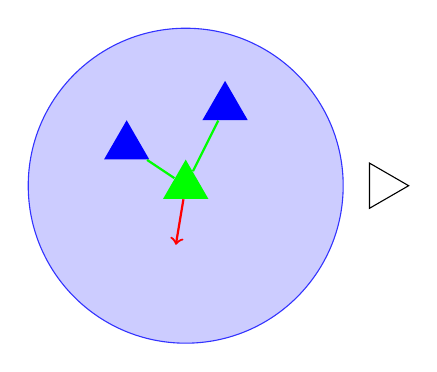
\begin{tikzpicture}
			      % Draw a semi-transparent blue circle with a dark border
			      \draw[fill=blue!20, draw=blue!80] (0,0) circle (2);
			      % Define a triangle shape
			      \node[regular polygon, regular polygon sides=3, minimum size=.5cm, fill,green] (t1) at (0,0) {};
			      \node[regular polygon, regular polygon sides=3, minimum size=.5cm, fill,blue] (t2) at (.5, 1) {};
			      \node[regular polygon, regular polygon sides=3, minimum size=.5cm, fill,blue] (t3) at (-.75, .5) {};
			      % Outside,rotated
			      \node[regular polygon, regular polygon sides=3, minimum size=.5cm, draw, rotate=30] (rotated) at (2.5,0) {};

			      \draw[green,thick] (t1) -- (t2);
			      \draw[green,thick] (t1) -- (t3);

			      \draw[red,thick,->] (t1) -- (-.125,-.75);
		      \end{tikzpicture}
	      \end{center}
	\item Maintain the same heading and speed as the neighboring boids.
	      \begin{center}
		      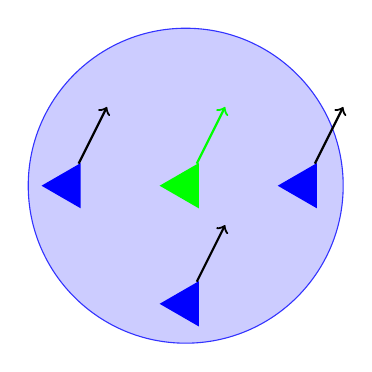
\begin{tikzpicture}
			      % Draw a semi-transparent blue circle with a dark border
			      \draw[fill=blue!20, draw=blue!80] (0,0) circle (2);
			      % Define a triangle shape
			      \node[regular polygon, regular polygon sides=3, minimum size=.5cm, fill,green,rotate=-30] (t1) at (0,0) {};
			      \node[regular polygon, regular polygon sides=3, minimum size=.5cm, fill,blue,rotate=-30] (t2) at (-1.5, 0) {};
			      \node[regular polygon, regular polygon sides=3, minimum size=.5cm, fill,blue,rotate=-30] (t3) at (1.5, 0) {};
			      \node[regular polygon, regular polygon sides=3, minimum size=.5cm, fill,blue,rotate=-30] (t4) at (0, -1.5) {};

			      \draw[green,thick,->] (t1) -- ++(.5, 1);
			      \draw[black,thick,->] (t2) -- ++(.5, 1);
			      \draw[black,thick,->] (t3) -- ++(.5, 1);
			      \draw[black,thick,->] (t4) -- ++(.5, 1);
		      \end{tikzpicture}
	      \end{center}
	\item Gravitate toward the center of the flock.
	      \begin{center}
		      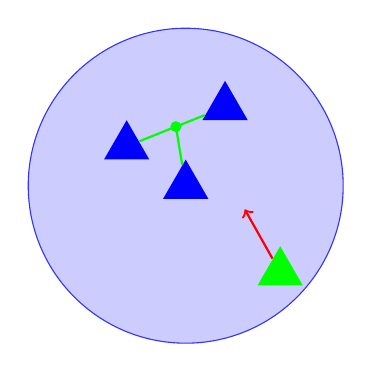
\begin{tikzpicture}
			      % Draw a semi-transparent blue circle with a dark border
			      \draw[fill=blue!20, draw=blue!80] (0,0) circle (2);
			      % Define a triangle shape
			      \node[regular polygon, regular polygon sides=3, minimum size=.5cm, fill,blue] (t1) at (0,0) {};
			      \node[regular polygon, regular polygon sides=3, minimum size=.5cm, fill,blue] (t2) at (.5, 1) {};
			      \node[regular polygon, regular polygon sides=3, minimum size=.5cm, fill,blue] (t3) at (-.75, .5) {};

			      \node[regular polygon, regular polygon sides=3, minimum size=.5cm, fill,green] (t4) at (1.2, -1.1) {};

			      \draw[green, thick] (t1) -- (-.125,.75);
			      \fill[green, thick] (-.125,.75) circle (2pt);
			      \draw[green,thick] (t2) -- (t3);

			      \draw[red,thick,->] (t4) -- (.75,-.3);
		      \end{tikzpicture}
	      \end{center}
\end{enumerate}

\subsection*{Basic boids implementation}

Each boid $B$ has the following properties:
\begin{enumerate}
	\item position - a vector in $ \mathbb{R}^2 $, denoted by $position(B)$,
	\item velocity - a vector in $ \mathbb{R}^2 $, denoted by $velocity(B)$,
	\item acceleration - a vector in $\mathbb{R}^2$; used exclusively
	      for the internal \\ computation of the boid's velocity and not for behavioral logic.
\end{enumerate}

\noindent With regards to behavioral logic, we also assign the following
attributes to all boids:
\begin{enumerate}
	\item perception radius (denoted by $r_P$)
	\item separation radius (denoted by $r_S$, also note that $ r_S < r_P $)
\end{enumerate}

\noindent The {\em Euclidean distance} (\ref{eq:eucl_dst}) is used for computing the distance between boids.
\begin{equation} \label{eq:eucl_dst}
	d(p, q) = \sqrt{(p_1-q_1)^2 + (p_2 - q_2)^2};\  p, q \in \mathbb{R}^2
\end{equation}
To avoid the computation of the costly square root of a real number, we utilize an equivalent formula
(\ref{eq:eucl_dst_sq}):
\begin{equation} \label{eq:eucl_dst_sq}
	d(p, q)^2 = (p_1-q_1)^2 + (p_2 - q_2)^2;\  p, q \in \mathbb{R}^2
\end{equation}

Each step of the simulation loop updates the direction of a boid, which is then applied to its acceleration,
determining the actual velocity for all boids.

The direction for collision avoidance, also known as {\em separation}, for boid $B$ is computed by the
following formula (\ref{eq:sum_dir_vectors}):
\begin{equation} \label{eq:sum_dir_vectors}
	direction = \sum_{i=1}^{n} position(B) - position(B_i)
\end{equation}
where $i$-th boid $B_i$ is a boid such that: $ d(position(B), position(B_i))^2 < r_S^2 $.
This effectively means that boid $B$ will move away (in the opposite direction) from the boids which are too near (closer than the specified $r_S$).

The direction for {\em alignment} for boid $B$ is computed as (\ref{eq:sum_align}):
\begin{equation} \label{eq:sum_align}
	direction = \left( \frac{\sum_{i=1}^{n} velocity(B_i)}{n} - velocity(B) \right) \mathbin{/} 8
\end{equation}
where $i$-th boid $B_i$ is a boid such that: $ d(position(B), position(B_i)^2 < r_P^2) $ (i.e., $B_i$ is $B$'s neighbour).
First, the average velocity of all neighboring boids is computed (denoted $v_{avg}$).
The velocity of current boid $B$ is then subtracted from $v_{avg}$, such that a vector in the direction
from $velocity(B)$ to $v_{avg}$ is obtained.
Adding such a vector to the $velocity(B)$ would result in $velocity(B)$ being equal to the $v_{avg}$.
Since this result is not desired, direction is lastly divided by a constant $8$.

The direction for {\em cohesion} for boid $B$ is computed like so (\ref{eq:sum_coh}):
\begin{equation} \label{eq:sum_coh}
	direction = \left( \frac{\sum_{i=1}^{n} \left(position(B_i) - position(B)\right)}{n} \right) \mathbin{/} 100
\end{equation}
where $i$-th boid $B_i$ is a boid such that: $ d(position(B), position(B_i)^2 < r_P^2) $ (i.e., $B_i$ is $B$'s neighbour).
In this formula a centroid to the neighboring boids is computed, which is then divided by $100$.
The reasoning behind the constant $100$ is that on every update, each boid would move $1\%$ towards the centroid.

\section*{Results}
We have successfully implemented the model described in the previous section.
Correct behaviour was confirmed with the help of special debug draw commands on top of the boids.
We present 3 screenshots of the simulation at steps $0, 50$ and $100$.
We can see that at first boids are in random positions, but as the simulation progresses, they start forming groups (\textbf{cohesion}) which generally go in the same direction (\textbf{alignment}).
Eventually, a single group is formed.

\begin{figure}[h]
	\centering
	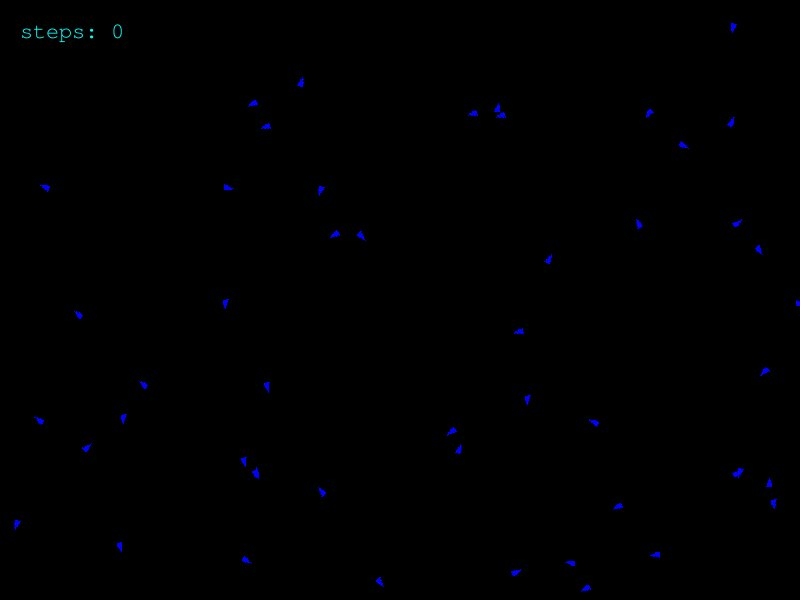
\includegraphics[width=0.8\linewidth]{boids_step_0.jpg}
	\caption{Boids simulation at step $0$}
\end{figure}
\begin{figure}[h]
	\centering
	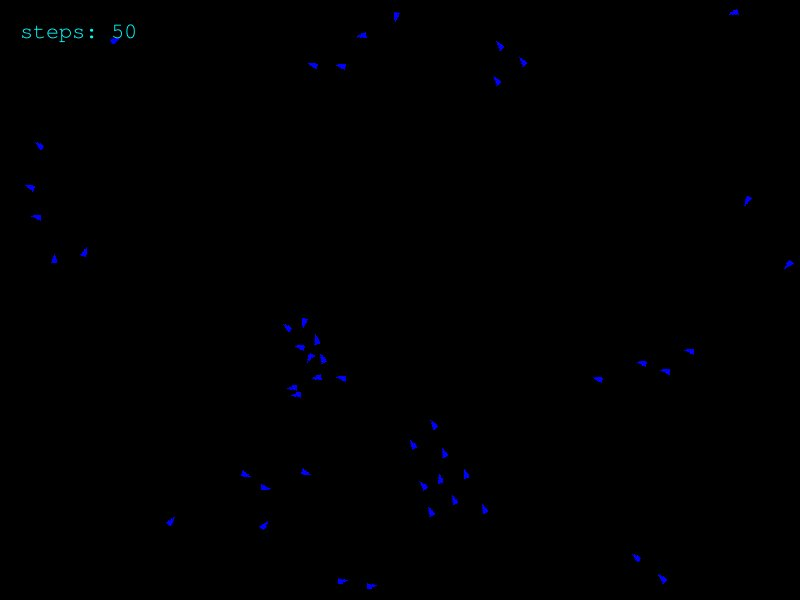
\includegraphics[width=0.8\linewidth]{boids_step_50.jpg}
	\caption{Boids simulation at step $50$}
\end{figure}
\begin{figure}[h]
	\centering
	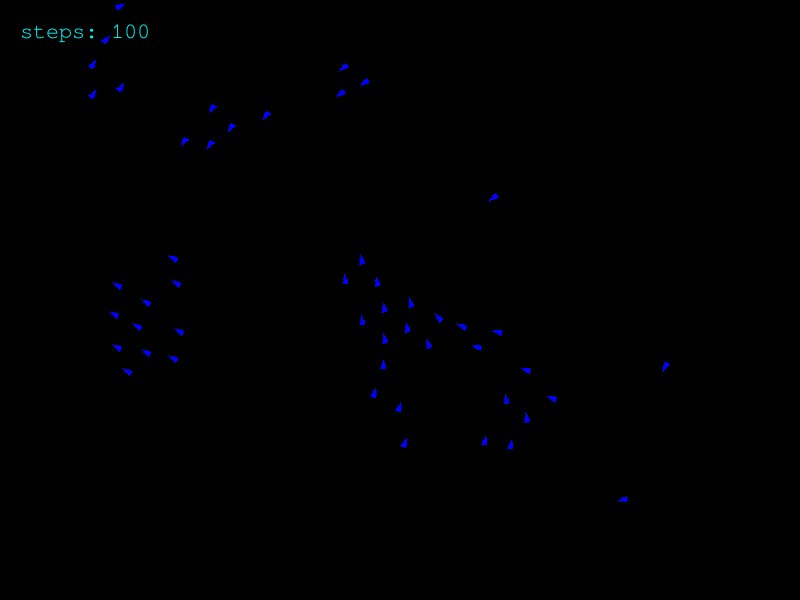
\includegraphics[width=0.8\linewidth]{boids_step_100.jpg}
	\caption{Boids simulation at step $100$}
\end{figure}

\newpage

\section*{Discussion}
This concludes the initial implementation of boids flocking simulation.
The following aspects remain to be implemented:
\begin{enumerate}
	\item use a more realistic perception (300 degrees instead of 360)
	\item take boid turn speed into account in computation
	\item take information propagation into account
	\item implement predators
	\item implement escape manuevers
	\item implement logic for determining success of predators
\end{enumerate}

\acknow{Matija Ojo: Initial boid implementation and report fixes, Miha Krajnc: Refactor boid implementation and report, Janez Kuhar: Initial version of report, Marko Adžaga: Report}

\showacknow % Display the acknowledgments section

% \pnasbreak splits and balances the columns before the references.
% If you see unexpected formatting errors, try commenting out this line
% as it can run into problems with floats and footnotes on the final page.
%\pnasbreak

\begin{multicols}{2}
	\section*{\bibname}
	% Bibliography
	\bibliography{bibliography}
\end{multicols}

\end{document}